\makeatletter
\parindent0pt

\cxset{style20a/.style={
 rule color=teal!90,
 block color=cyan,
 name=chapter,
 numbering = arabic,
 number font-size=\HHUGE,
 number color= white,
 number font-family=\sffamily,
 number font-weight=\bfseries,
 number before={\hbox to 0pt{\vbox to -10pt{\colorbox{\blockcolor@cx}{\rule{0pt}{70pt}\HHUGE \color{\blockcolor@cx}1331}}}\vskip1pt\vskip10pt\relax\hspace{2.5em}},
 number after=\hspace{3em},
 number dot={ },
 number position=rightname,
 chapter font-family=\rmfamily,
 chapter font-weight=\normalfont,
 chapter font-size=\large,
 chapter before=,
 chapter after={\hskip0pt},
 chapter color=white,
 title beforeskip={},
 title afterskip={\vspace*{30pt}\par}, 
 title before={\hskip0.2em},
 title after={\par\vspace{0pt}\color{\rulecolor@cx}\rule{\textwidth}{5pt}},
 title font-family=\sffamily,
 title font-color= black!90,
 title font-weight=\bfseries,
 title font-size=\HUGE,
 section color=teal,
 section font-family=\sffamily,
 section font-weight=\bfseries,
 section font-shape=\upshape\color{teal},
 section indent=-10pt,
 header style=plain}}

\cxset{style20}
\parindent1em
\chapter{STYLE 20}

\lettrine{\textcolor{teal}{T}}{his} style is probably useful in some corporate environment. The layout has been defined traditionally using boxes and skips and can perhaps be improved tremendously via TikZ. I selected this layout from a book titled \textit{Manufacturing at Warp Speed}, Eli Schragenheim, H. William Dettmer, 2001. The original book's chapter header is not coloured. We will use this example to define color schemes and themes.
\index{color schemes}\index{themes}.
\medskip
\begin{figure}[ht]
\centering
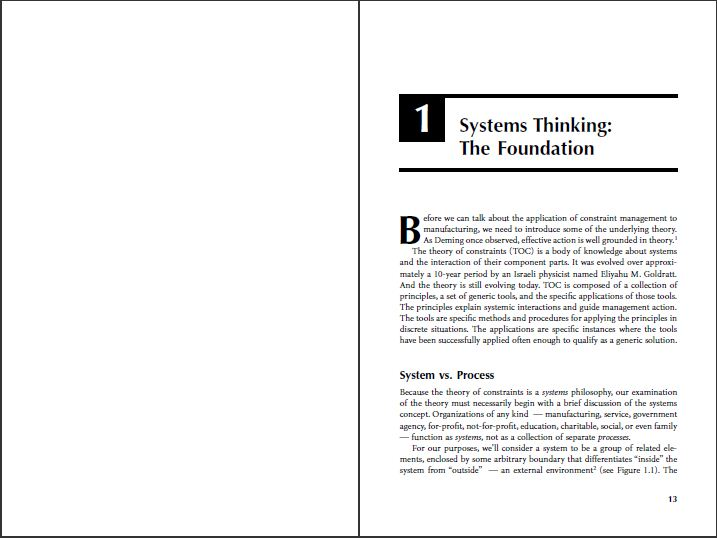
\includegraphics[width=0.7\textwidth]{./chapters/chapter20.png}
\end{figure}

\section{Creating themes}
The strategy we use to define themes, especially if based on color changes is to define commands to generate them. This way one could define a number of themes fairly quickly.

\section{Adding templates and themes to a library}
Templates that have a lot of themes can be considered libraries and can be loaded with the package. (See the section on libraries).

\begin{texexample}{}{}
\cxset{chapter opening=anywhere}
\newcommand\maketheme[3][style20]{
\cxset{#1 #2/.style={#1,#3 }}}
\maketheme[style20]{black}{rule color=black,block color=black,}
\maketheme[style20]{blue}{rule color=theblue,block color=theblue,}
\maketheme[style20]{blue}{rule color=theblue,block color=theblue,}
\maketheme[style20]{orange}{rule color=orange,block color=orange,}
\cxset{style20 black}
\chapter{A Test}
\cxset{style20 blue}
\chapter{A Test}
\cxset{style20 orange}
\chapter{A Test}
\end{texexample}

\begin{texexample}{}{}
\fboxrule0pt\fboxsep0pt
\colorbox{teal}{\fbox{\parbox[b]{3cm}{%
\vbox to 0pt{\hbox to 3cm{\hfill\large\itshape\color{white} Chapter\hfill}}
\vbox{}%
\hbox to 3cm{\hfill \color{white}\sffamily\bfseries\HHUGE39\rule{0pt}{60pt}}
\hbox to 3cm{\rule{0pt}{40pt}}
}}}\hspace{0.5em}
\fbox{\parbox[b]{13cm}{%
\huge\color{teal} Paradoxical functional facilitation\\[-1pt] and recovery in neurological\\[-1pt]
 and psychiatric conditions\par
\medskip
\vspace*{20pt}
\color{black}
\large Dr Yiannis Lazaridegj
}}

\end{texexample}


\newcommand\allbluechapter[2][]{%
\fboxrule0pt\fboxsep0pt%
\hspace*{-1em}\fbox{\colorbox{theblock}{\fbox{\parbox[b]{3cm}{%
\vbox to 0pt{\hbox to 3cm{\hfill\large\itshape\color{white} Chapter\hfill}}
\vbox{}%
\hbox to 3cm{\hfill \color{white}\sffamily\bfseries\HHUGE\thechapter\rule{0pt}{60pt}}
\hbox to 3cm{\rule{0pt}{40pt}}%
}}}\hspace{1.5em}
\fbox{\parbox[b]{10cm}{%
\huge\color{teal} #2\par
\medskip
\vspace*{10pt}
\color{black}
\large \authorblockformat@cx\authorblock@cx
}}}
\vspace{25pt}

\thispagestyle{plain}
}
\clearpage


\@specialtrue
\cxset{custom=allbluechapter,
         header style=plain, 
         chapter opening=any,
         chapter color= white,
         chapter font-weight=upshape,
         section align=left,
         subsection numbering=none,
         subsection color=teal,
         subsection font-weight=\bfseries,
         subsection font-shape=\upshape,
         subsection indent=-10pt,
         author block=true,
         author block format=\bfseries\normalfont\raggedright,
         author names={Dr Yiannis Lazarides, Maria Lazarides and Athena Lazarides}}
\renewsubsection\renewsection
\parindent1em
\chapter[Paradoxical facilitation]{Paradoxical functional facilitation\\ and recovery in neurological\\
 and psychiatric conditions}

\section{Introduction}
\lorem

\section{Author Block Formatting}

Each chapter of the book carries the names of its authors, which is typeset as shown above. The standard available fields for author blocks are programmed in the special template. The full settings are shown in Example .
\medskip

\noindent\begin{tcolorbox}
\begin{lstlisting}
\@specialtrue
\cxset{custom=allbluechapter,
         header style=plain, 
         chapter opening=any,
         author block=true,
         author block format=\bfseries\normalfont\raggedright,
         author names=Dr Yiannis Lazarides, Maria Lazarides and Athena Lazarides}
\chapter{Paradoxical functional facilitation...}
\end{lstlisting}
\end{tcolorbox}

Remember that it is also possible to add the author with the command \cs{addauthor} or its alias macro \cs{addauthors}. Cases where people can make mistakes are normally aliased to avoid common errors.

\section{Key value interface}
\subsection{General keys}
All keys for chapters chapters can be used in the template and toc.
Additional keys are described below.


\subsection{Other formatting hooks}

When a special template is designed it is prudent to provide hooks for minor tweaks. This way it is unecessary to modify the code of a special template for such changes. Keys have been provided for all the struts etc.
All normal keys can be used, such as font selection, spacing etc.

\lipsum
